\documentclass[mathserif,xcolor=dvipsnames,hyperref={bookmarks=true}]{beamer}
%\documentclass[mathserif,xcolor=dvipsnames,handout]{beamer}
%\usepackage{listings}
\usepackage[scaled]{helvet}
\usepackage{eulervm}
\usepackage{listings}
\usepackage{courier}
\usepackage{xmpincl}  % http://www.ctan.org/tex-archive/macros/latex/contrib/xmpincl/
\usepackage{listings}
\includexmp{byncsa}
\usepackage[binary,amssymb]{SIunits}
\usefonttheme{structurebold}
\usecolortheme[named=Maroon]{structure}
\usetheme{Antibes}
\usecolortheme{lily}
\useoutertheme{infolines}
\setbeamertemplate{navigation symbols}{}


% Check this for automating the creation of different files: slides, handouts, etc...
% http://www.pletscher.org/writings/latex/Makefile
% http://www.pletscher.org/writings/latex/beamer.php

% Do this if handouts...
%\usepackage{pgfpages}
%\pgfpagesuselayout{2 on 1}[letterpapper,border shrink=5mm]
%\mode<handout>{\setbeamercolor{background canvas}{bg=black!5}}

\usepackage{default}

\title[Creative Commons]{Creative Commons}
\subtitle{Including a Usage Management Example in Ruby}
\author[Matthew Bohnsack]{Matthew Bohnsack}
\institute[UNM]{University of New Mexico\\Albuquerque, New Mexico USA\\[2ex]\texttt{mbohnsac@unm.edu}}
\date{Friday March 25, 2011}

\newcommand{\putat}[3]{\begin{picture}(0,0)(0,0)\put(#1,#2){#3}\end{picture}}


\lstset{language=bash,rulesepcolor=\color{Gray},frame=shadowbox,basicstyle=\tiny\ttfamily}

\begin{document}

%%%%%%%%%%%%%%%%%%%%%%%%%%%%%%%%%%%%%%%%%%%%%%%%%%%%%%%%%%%%%%%%%%%%%
% Title
%%%%%%%%%%%%%%%%%%%%%%%%%%%%%%%%%%%%%%%%%%%%%%%%%%%%%%%%%%%%%%%%%%%%%
\begin{frame}
    \titlepage
    \begin{center}
        
\includegraphics[width=0.24\textwidth]{resources/logos/UNM/UNM_logo_PMS200C.pdf}
        \hspace{0.5in}
        
\includegraphics[width=0.24\textwidth]{resources/cc/cc_logo.pdf}
    \end{center}
\end{frame}


%%%%%%%%%%%%%%%%%%%%%%%%%%%%%%%%%%%%%%%%%%%%%%%%%%%%%%%%%%%%%%%%%%%%%
\section{Creative Commons}
%%%%%%%%%%%%%%%%%%%%%%%%%%%%%%%%%%%%%%%%%%%%%%%%%%%%%%%%%%%%%%%%%%%%%
\begin{frame}[t]
    \tableofcontents[currentsection,hideallsubsections]
\end{frame}

    \subsection{Overview}
    %%%%%%%%%%%%%%%%%%%%%%%%%%%%%%%%%%%%%%%%%%%%%%%%%%%%%%%%%%%%%%%%%%%%%
    \begin{frame}[t]
        \frametitle{Overview}
        \begin{itemize}
            \item A nonprofit organization that works to increase the amount of
                  creativity available in ``the commons''
            \item Provides free, easy-to-use legal tools that provide a simple,
                  standardized way to pre-clear usage rights to creative work for copyright owners
            \item Lets copyright holders easily change from default of ``all
                  rights reserved'' to ``some rights reserved''
            \item Not an alternative to copyright
            \item Applies on top of copyright
            \item Guidelines for marking text, images, audio, and video
            \item Guidelines for publishing via a file sharing network or social networking site
            \item Some support for embedding license information as meta-data within digital files
        \end{itemize}
    \end{frame}

    \begin{frame}[t]
        \frametitle{Overview (cont.)}
        \begin{itemize}
            \item Not changable or revocable
            \item I.e., once someone has received a copy, the work is perpetually licensed under the license it was received under
            \item View is always permissible under CC
        \end{itemize}
    \end{frame}

    \subsection{Three Layers}
    %%%%%%%%%%%%%%%%%%%%%%%%%%%%%%%%%%%%%%%%%%%%%%%%%%%%%%%%%%%%%%%%%%%%%
    \begin{frame}[t]
        \frametitle{Three Layers}
            \begin{itemize}
                \item Machine Readable (CC Rights Expression Language - CC REL)
                \item Human Readable (Commons Deed)
                \item Legal Code (Lawyer Readable)
            \end{itemize}
        \begin{center}
          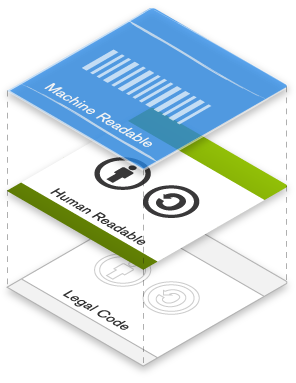
\includegraphics[width=0.4\textwidth]{figures/license_layers.png}
        \end{center}
    \end{frame}

    \subsection{Licenses}
    %%%%%%%%%%%%%%%%%%%%%%%%%%%%%%%%%%%%%%%%%%%%%%%%%%%%%%%%%%%%%%%%%%%%%
    \begin{frame}[t]
        \frametitle{Licenses}
        \begin{itemize}
            \item Six licenses are provided by CC, not including the
             complications of locale-specific licenses, license versions, or CC0 (Public
             Domain ``no rights reserved'')
            \begin{enumerate}
              \item 
\includegraphics[width=0.1\textwidth]{resources/cc/by.pdf}\ Attribution / CC BY
              \item 
\includegraphics[width=0.1\textwidth]{resources/cc/by_sa.pdf}\ Attribution-ShareAlike / CC BY-SA
              \item 
\includegraphics[width=0.1\textwidth]{resources/cc/by_nd.pdf}\ Attribution-NoDerivs / CC BY-ND
              \item 
\includegraphics[width=0.1\textwidth]{resources/cc/by_nc.pdf}\ Attribution-NonCommercial / CC BY-NC
              \item 
\includegraphics[width=0.1\textwidth]{resources/cc/by_nc_sa.pdf}\ Attribution-NonCommercial-ShareAlike / CC BY-NC-SA
              \item 
\includegraphics[width=0.1\textwidth]{resources/cc/by_nc_nd.pdf}\ Attribution-NonCommercial-NoDerivs / CC BY-NC-ND
            \end{enumerate}
            \item Non-exclusive licenses, yielding CC+: \texttt{http://wiki.creativecommons.org/CCPlus} \\
              
\includegraphics[width=0.1\textwidth]{resources/cc/by_nc_sa.pdf} +
\includegraphics[width=0.1\textwidth]{resources/cc/CommercialLicenseButton.pdf}
        \end{itemize}
    \end{frame}

% https://creativecommons.org/about/downloads

    % 1 %%%%%%%%%%%%%%%%%%%%%%%%%%%%%%%%%%%%%%%%%%%%%%%%%%%%%%%%%%%%%%%%%%%%
    \begin{frame}[t]
        \frametitle{Attribution}
        
\includegraphics[width=0.1\textwidth]{resources/cc/by.pdf}\  This
license lets others distribute, remix, tweak, and build upon your work, even
commercially, as long as they credit you for the original creation.  This is
the most accommodating of the licenses offered.  Recommended for maximum
dissemination and use of licensed materials.
\vspace{0.1in}
        \begin{itemize}
            \item You are free:
            \begin{itemize}
                \item 
\includegraphics[width=0.03\textwidth]{resources/cc/share.pdf}\ \textbf{to Share} -- to copy, distribute, and transmit the work
                \item 
\includegraphics[width=0.03\textwidth]{resources/cc/remix.pdf}\ \textbf{to Remix} -- to adapt the work
            \end{itemize}
            \item Under the following conditions:
            \begin{itemize}
                \item 
\includegraphics[width=0.03\textwidth]{resources/cc/bigby.pdf}\ \textbf{Attribution} -- You must attribute the work in
                the manner specified by the author or licensor (but not in any
                way that suggests that they endorse you or your use of the work).
            \end{itemize}
        \end{itemize}
    \end{frame}

    % 2 %%%%%%%%%%%%%%%%%%%%%%%%%%%%%%%%%%%%%%%%%%%%%%%%%%%%%%%%%%%%%%%%%%%%
    \begin{frame}[t]
        \frametitle{Attribution-ShareAlike}
        
\includegraphics[width=0.1\textwidth]{resources/cc/by_sa.pdf}\
This license lets others remix, tweak, and build upon your work even for
commercial purposes, as long as they credit you and license their new creations
under the identical terms. This license is often compared to free
and open source software licenses. All new works based on yours will carry the
same license, so any derivatives will also allow commercial use.
\vspace{0.1in}
        \begin{itemize}
            \item You are free:
            \begin{itemize}
                \item 
\includegraphics[width=0.03\textwidth]{resources/cc/share.pdf}\ \textbf{to Share} -- to copy, distribute, and transmit the work
                \item 
\includegraphics[width=0.03\textwidth]{resources/cc/remix.pdf}\ \textbf{to Remix} -- to adapt the work
            \end{itemize}
            \item Under the following conditions:
            \begin{itemize}
                \item 
\includegraphics[width=0.03\textwidth]{resources/cc/bigby.pdf}\ \textbf{Attribution} -- You must attribute the work in the manner specified by the author or licensor (but not in any way that suggests that they endorse you or your use of the work).
                %\item 
\includegraphics[width=0.03\textwidth]{resources/cc/nd.pdf}\ \textbf{No Derivative Works} -- You may not alter, transform, or build upon this work.
                \item 
\includegraphics[width=0.03\textwidth]{resources/cc/sa.pdf}\ \textbf{Share Alike} -- If you alter, transform, or build upon this work, you may distribute the resulting work only under the same or similar license to this one.
            \end{itemize}
        \end{itemize}
    \end{frame}

    % 3 %%%%%%%%%%%%%%%%%%%%%%%%%%%%%%%%%%%%%%%%%%%%%%%%%%%%%%%%%%%%%%%%%%%%
    \begin{frame}[t]
        \frametitle{Attribution-NoDerivs}
        
\includegraphics[width=0.1\textwidth]{resources/cc/by_nd.pdf}\ This
        license allows for redistribution, commercial and non-commercial, as long as it
        is passed along unchanged and in whole, with credit to you.
\vspace{0.1in}
        \begin{itemize}
            \item You are free:
            \begin{itemize}
                \item 
\includegraphics[width=0.03\textwidth]{resources/cc/share.pdf}\ \textbf{to Share} -- to copy, distribute, and transmit the work
                %\item 
\includegraphics[width=0.03\textwidth]{resources/cc/remix.pdf}\ \textbf{to Remix} -- to adapt the work
            \end{itemize}
            \item Under the following conditions:
            \begin{itemize}
                \item 
\includegraphics[width=0.03\textwidth]{resources/cc/bigby.pdf}\ \textbf{Attribution} -- You must attribute the work in the manner specified by the author or licensor (but not in any way that suggests that they endorse you or your use of the work).
                \item 
\includegraphics[width=0.03\textwidth]{resources/cc/nd.pdf}\ \textbf{No Derivative Works} -- You may not alter, transform, or build upon this work.
            \end{itemize}
        \end{itemize}
    \end{frame}

    % 4 %%%%%%%%%%%%%%%%%%%%%%%%%%%%%%%%%%%%%%%%%%%%%%%%%%%%%%%%%%%%%%%%%%%%
    \begin{frame}[t]
        \frametitle{Attribution-NonCommercial}
        
\includegraphics[width=0.1\textwidth]{resources/cc/by_nc.pdf}\ This license lets others remix, tweak, and build upon your work
non-commercially, and although their new works must also acknowledge you and be
non-commercial, they don't have to license their derivative works on the same
terms.
\vspace{0.1in}
        \begin{itemize}
            \item You are free:
            \begin{itemize}
                \item 
\includegraphics[width=0.03\textwidth]{resources/cc/share.pdf}\ \textbf{to Share} -- to copy, distribute, and transmit the work
                \item 
\includegraphics[width=0.03\textwidth]{resources/cc/remix.pdf}\ \textbf{to Remix} -- to adapt the work
            \end{itemize}
            \item Under the following conditions:
            \begin{itemize}
                \item 
\includegraphics[width=0.03\textwidth]{resources/cc/bigby.pdf}\ \textbf{Attribution} -- You must attribute the work in the manner specified by the author or licensor (but not in any way that suggests that they endorse you or your use of the work).
                %\item 
\includegraphics[width=0.03\textwidth]{resources/cc/nd.pdf}\ \textbf{No Derivative Works} -- You may not alter, transform, or build upon this work.
                \item 
\includegraphics[width=0.03\textwidth]{resources/cc/nc.pdf}\ \textbf{Noncommercial} -- You may not use this work for commercial purposes.
            \end{itemize}
        \end{itemize}
    \end{frame}

    % 5 %%%%%%%%%%%%%%%%%%%%%%%%%%%%%%%%%%%%%%%%%%%%%%%%%%%%%%%%%%%%%%%%%%%%
    \begin{frame}[t]
        \frametitle{Attribution-NonCommercial-ShareAlike}
        
\includegraphics[width=0.1\textwidth]{resources/cc/by_nc_sa.pdf}\
This license lets others remix, tweak, and build upon your work non-commercially, as long as they credit you and license their new creations under the identical terms.
\vspace{0.1in}
        \begin{itemize}
            \item You are free:
            \begin{itemize}
                \item 
\includegraphics[width=0.03\textwidth]{resources/cc/share.pdf}\ \textbf{to Share} -- to copy, distribute, and transmit the work
                \item 
\includegraphics[width=0.03\textwidth]{resources/cc/remix.pdf}\ \textbf{to Remix} -- to adapt the work
            \end{itemize}
            \item Under the following conditions:
            \begin{itemize}
                \item 
\includegraphics[width=0.03\textwidth]{resources/cc/bigby.pdf}\ \textbf{Attribution} -- You must attribute the work in the manner specified by the author or licensor (but not in any way that suggests that they endorse you or your use of the work).
                %\item 
\includegraphics[width=0.03\textwidth]{resources/cc/nd.pdf}\ \textbf{No Derivative Works} -- You may not alter, transform, or build upon this work.
                \item 
\includegraphics[width=0.03\textwidth]{resources/cc/nc.pdf}\ \textbf{Noncommercial} -- You may not use this work for commercial purposes.
                \item 
\includegraphics[width=0.03\textwidth]{resources/cc/sa.pdf}\ \textbf{Share Alike} -- If you alter, transform, or build upon this work, you may distribute the resulting work only under the same or similar license to this one.
            \end{itemize}
        \end{itemize}

    \end{frame}

    % 6 %%%%%%%%%%%%%%%%%%%%%%%%%%%%%%%%%%%%%%%%%%%%%%%%%%%%%%%%%%%%%%%%%%%%
    \begin{frame}[t]
        \frametitle{Attribution-NonCommercial-NoDerivs}
        
\includegraphics[width=0.1\textwidth]{resources/cc/by_nc_nd.pdf}\
This license is the most restrictive of the six main licenses, only allowing others to download your works and share them with others as long as they credit you, but they can't change them in any way or use them commercially.
\vspace{0.1in}
        \begin{itemize}
            \item You are free:
            \begin{itemize}
                \item 
\includegraphics[width=0.03\textwidth]{resources/cc/share.pdf}\ \textbf{to Share} -- to copy, distribute, and transmit the work
                %\item 
\includegraphics[width=0.03\textwidth]{resources/cc/remix.pdf}\ \textbf{to Remix} -- to adapt the work
            \end{itemize}
            \item Under the following conditions:
            \begin{itemize}
                \item 
\includegraphics[width=0.03\textwidth]{resources/cc/bigby.pdf}\ \textbf{Attribution} -- You must attribute the work in the manner specified by the author or licensor (but not in any way that suggests that they endorse you or your use of the work).
                \item 
\includegraphics[width=0.03\textwidth]{resources/cc/nc.pdf}\ \textbf{Noncommercial} -- You may not use this work for commercial purposes.
                \item 
\includegraphics[width=0.03\textwidth]{resources/cc/nd.pdf}\ \textbf{No Derivative Works} -- You may not alter, transform, or build upon this work.
                %\item 
\includegraphics[width=0.03\textwidth]{resources/cc/sa.pdf}\ \textbf{Share Alike} -- If you alter, transform, or build upon this work, you may distribute the resulting work only under the same or similar license to this one.
            \end{itemize}
        \end{itemize}

    \end{frame}

    \begin{frame}[t]
        \frametitle{Select License Example}
        \begin{center}
          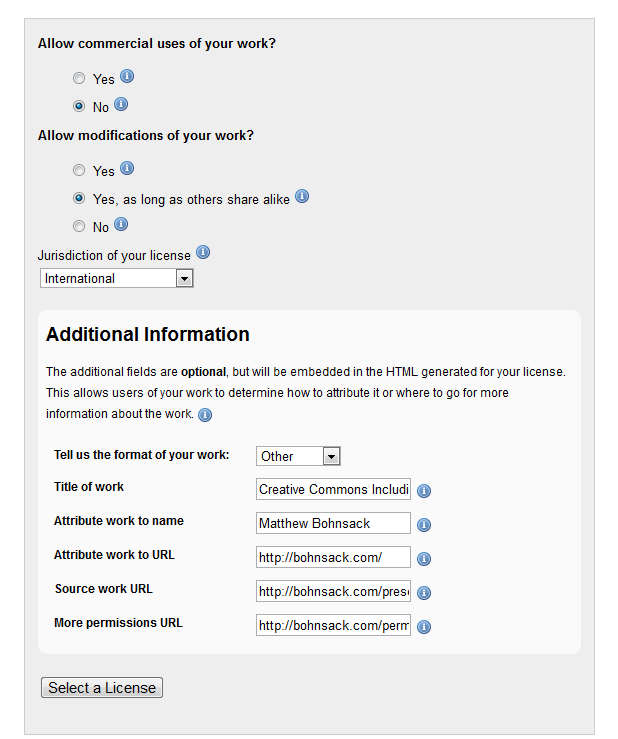
\includegraphics[width=0.5\textwidth]{figures/selectlicense.png}
        \end{center}
    \end{frame}

    \begin{frame}[t]
        \frametitle{View License}
        \begin{center}
          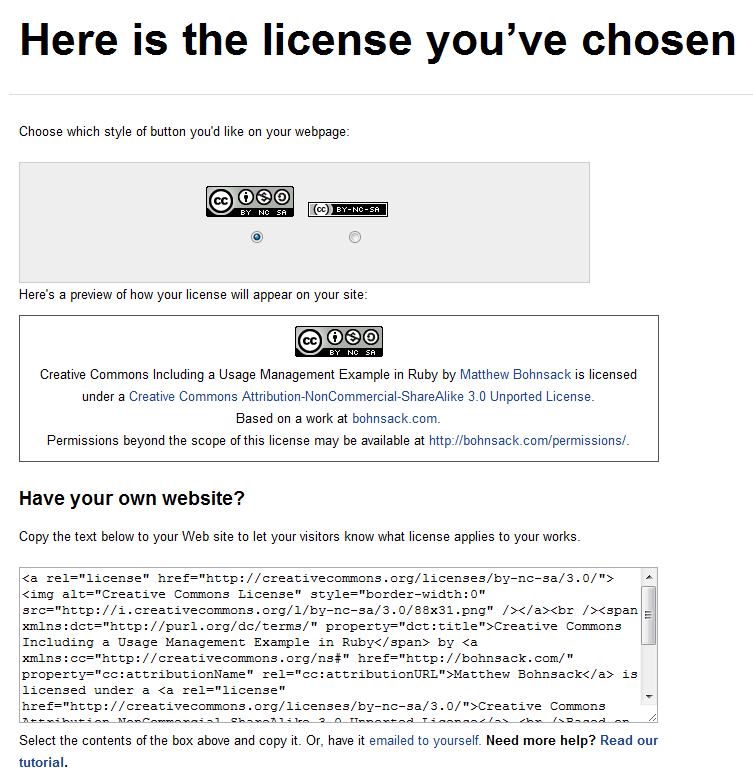
\includegraphics[width=0.55\textwidth]{figures/hereislicense.png}
        \end{center}
    \end{frame}

    \begin{frame}[t]
        \frametitle{Terms for Derivative Works or Adaptation}
        \begin{center}
          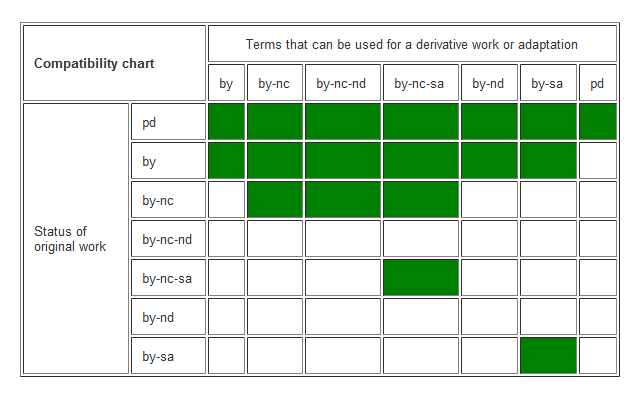
\includegraphics[width=0.8\textwidth]{figures/terms_for_derivative_work_or_adaptation.png}
        \end{center}
    \end{frame}

    \begin{frame}[t]
        \frametitle{Collecting CC Works Together}
        \begin{center}
          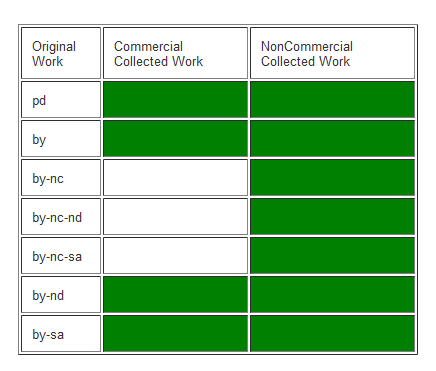
\includegraphics[width=0.7\textwidth]{figures/collecting_cc_works_together.png}
        \end{center}
    \end{frame}

%%%%%%%%%%%%%%%%%%%%%%%%%%%%%%%%%%%%%%%%%%%%%%%%%%%%%%%%%%%%%%%%%%%%%
\section{CC REL}
%%%%%%%%%%%%%%%%%%%%%%%%%%%%%%%%%%%%%%%%%%%%%%%%%%%%%%%%%%%%%%%%%%%%%
\begin{frame}[t]
    \tableofcontents[currentsection,hideallsubsections]
\end{frame}

    \subsection{CC REL: The Creative Commons Rights Expression Language}
    %%%%%%%%%%%%%%%%%%%%%%%%%%%%%%%%%%%%%%%%%%%%%%%%%%%%%%%%%%%%%%%%%%%%%
    \begin{frame}[t]
        \frametitle{CC REL}
        \begin{itemize}
            \item The Creative Commons Rights Expression Language
            \item RDFa (Resource Description Framework in attributes) for HTML Web pages and resources referenced therein
            \item XMP (Extensible Metadata Platform) for stand-alone media
            \item \texttt{http://wiki.creativecommons.org/CC\_REL}
        \end{itemize}
    \end{frame}

    \subsection{RDFa for HTML}
    %%%%%%%%%%%%%%%%%%%%%%%%%%%%%%%%%%%%%%%%%%%%%%%%%%%%%%%%%%%%%%%%%%%%%
\begin{frame}[fragile]
\frametitle{Example: RDFa for HTML}
\lstinputlisting[language=HTML]{examples/RDFaExample.html}
\end{frame}

    \subsection{XMP for Stand-Alone Media}
    %%%%%%%%%%%%%%%%%%%%%%%%%%%%%%%%%%%%%%%%%%%%%%%%%%%%%%%%%%%%%%%%%%%%%
    \begin{frame}[t]
        \frametitle{Example: XMP for Stand-Alone Media}
        \begin{itemize}
            \item \LaTeX\ package on CTAN (\texttt{xmpincl})
        \end{itemize}
        \begin{center}
            \includegraphics[width=0.7\textwidth]{figures/embedded_xmp.png}
        \end{center}
    \end{frame}

%%%%%%%%%%%%%%%%%%%%%%%%%%%%%%%%%%%%%%%%%%%%%%%%%%%%%%%%%%%%%%%%%%%%%
\section{Usage Management Example in Ruby}
%%%%%%%%%%%%%%%%%%%%%%%%%%%%%%%%%%%%%%%%%%%%%%%%%%%%%%%%%%%%%%%%%%%%%
\begin{frame}[t]
    \tableofcontents[currentsection,hideallsubsections]
\end{frame}

    \subsection{Book Class}
    %%%%%%%%%%%%%%%%%%%%%%%%%%%%%%%%%%%%%%%%%%%%%%%%%%%%%%%%%%%%%%%%%%%%%
\begin{frame}[fragile]
\frametitle{Book Class}
\lstinputlisting[language=Ruby,showspaces=false,showstringspaces=false]{code/book.rb}
\end{frame}

    \subsection{CC Licensed Mix-in}
    %%%%%%%%%%%%%%%%%%%%%%%%%%%%%%%%%%%%%%%%%%%%%%%%%%%%%%%%%%%%%%%%%%%%%
\begin{frame}[fragile]
\frametitle{CC Licensed Mix-in}
\lstinputlisting[language=Ruby,showspaces=false,showstringspaces=false]{code/for_pres/cc_licensed1.rb}
\end{frame}

    \subsection{CC Licensed Mix-in (cont.)}
    %%%%%%%%%%%%%%%%%%%%%%%%%%%%%%%%%%%%%%%%%%%%%%%%%%%%%%%%%%%%%%%%%%%%%
\begin{frame}[fragile]
\frametitle{CC Licensed Mix-in (cont.)}
\lstinputlisting[language=Ruby,showspaces=false,showstringspaces=false]{code/for_pres/cc_licensed2.rb}
\end{frame}

    \subsection{CC Licensed Mix-in (cont.)}
    %%%%%%%%%%%%%%%%%%%%%%%%%%%%%%%%%%%%%%%%%%%%%%%%%%%%%%%%%%%%%%%%%%%%%
\begin{frame}[fragile]
\frametitle{CC Licensed Mix-in (cont.)}
\lstinputlisting[language=Ruby,showspaces=false,showstringspaces=false]{code/for_pres/cc_licensed3.rb}
\end{frame}

    \subsection{Unit Tests}
    %%%%%%%%%%%%%%%%%%%%%%%%%%%%%%%%%%%%%%%%%%%%%%%%%%%%%%%%%%%%%%%%%%%%%
\begin{frame}[fragile]
\frametitle{Unit Tests}
\lstinputlisting[showspaces=false,showstringspaces=false]{code/test/for_pres/ts_cc1.rb}
\end{frame}

    \subsection{Unit Tests (cont.)}
    %%%%%%%%%%%%%%%%%%%%%%%%%%%%%%%%%%%%%%%%%%%%%%%%%%%%%%%%%%%%%%%%%%%%%
\begin{frame}[fragile]
\frametitle{Unit Tests}
\lstinputlisting[showspaces=false,showstringspaces=false]{code/test/for_pres/ts_cc2.rb}
\end{frame}

    \subsection{Unit Tests (cont.)}
    %%%%%%%%%%%%%%%%%%%%%%%%%%%%%%%%%%%%%%%%%%%%%%%%%%%%%%%%%%%%%%%%%%%%%
\begin{frame}[fragile]
\frametitle{Unit Tests}
\lstinputlisting[showspaces=false,showstringspaces=false]{code/test/for_pres/ts_cc3.rb}
\end{frame}

    \subsection{Test Output}
    %%%%%%%%%%%%%%%%%%%%%%%%%%%%%%%%%%%%%%%%%%%%%%%%%%%%%%%%%%%%%%%%%%%%%
\begin{frame}[fragile]
\frametitle{Test Output}
\lstinputlisting[showspaces=false,showstringspaces=false]{code/test_output}
\end{frame}

\end{document}
